\chapter{Parallel Programming Models}
In this section different parallel programming models are discussed, together with their advantages and disadvantages.

\begin{figure}
	\centering
	\subfloat[Shared Memory] {
		\input{Tikz/SharedMemory}
		\label{fig:shared_memory}
	}
	$\hspace{36pt}$
	\subfloat[Distributed Memory] {
		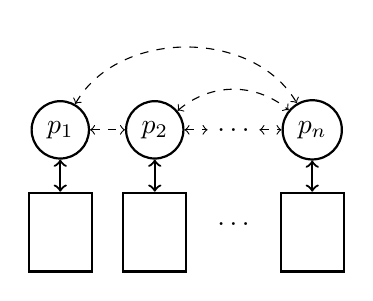
\begin{tikzpicture}
\node[circle, thick, draw] (v1) at (-0.2,0.8) {$p_1$};
\node[circle, thick, draw] (v3) at (1,0.8) {$p_2$};
\node (v7) at (2,0.8) {$\dots$};
\node at (2,-0.4) {$\dots$};
\node[circle, thick, draw] (v5) at (3,0.8) {$p_n$};

\node (v2) at (-0.2,-0.11) {};
\node (v4) at (1,-0.11) {};
\node (v6) at (3,-0.11) {};

\draw[thick] (-0.6,0) rectangle (0.2,-1);
\draw[thick]  (0.6,0) rectangle (1.4,-1);
\draw[thick]  (2.6,0) rectangle (3.4,-1);

\draw[<->, thick]  (v1) edge (v2);
\draw[<->, thick]  (v3) edge (v4);
\draw[<->, thick]  (v5) edge (v6);

\draw[<->, dashed]  (v1) edge (v3);
\draw[<->, dashed]  (v3) edge (v7);
\draw[<->, dashed]  (v7) edge (v5);
\draw[<->, dashed]  (v3) edge [bend left=40 ] (v5) ;
\draw[<->, dashed]  (v1) edge [bend left=60 ] (v5);

\end{tikzpicture}
		\label{fig:distributed_memory}
	}

	\caption{Here $n$ processes $p_1, \dots, p_n$ are displayed in a \emph{Shared Memory} and a \emph{Distributed Memory} setting. Dashed edges represent communication links between processes.}
	\label{fig:shared_distributed_memory}
\end{figure}

\section{Shared Memory Architecture}
In a \emph{Shared Memory Architecture (SMA)}, all processes work in a shared address space, like shown in Figure \ref{fig:shared_memory}. Note that interprocess communication is done implicitly, since every process can access the entire address space.

Since the entire available memory can be accessed via a shared address space, the shared memory model simplifies programming. Algorithms with challenging data dependencies can be modelled elegantly in shared memory. A disadvantage is that data locality is not taken into account, because processes are not aware where data resides. This could bring performance penalties.

\subsection{NUMA}
An example of a shared memory architecture is \emph{Non-Uniform Memory Access (NUMA)}, a model used in computer systems with multiple CPUs. In NUMA every CPU has a local memory and and every CPU can access memory local to other CPUs via a shared address space. Some parts of the address space are on different buses than others, so different parts of the address space may differ in performance. This makes memory accesses non-uniformly.

NUMA is contrasted with \emph{Uniform Memory Access (UMA)}, in which all CPUs share the same physical memory uniformly.

\subsection{SMP}
Another example of shared memory architectures is the \emph{Symmetric Multiprocessing (SMP)} architecture. In SMP all CPUs access memory via the same shared memory bus. Memory-intensive algorithms generally perform better under the NUMA architecture, since the single memory bus in SMP can easily become a performance bottleneck.

\section{Distributed Memory Architecture}
Figure \ref{fig:distributed_memory} shows a \emph{Distributed Memory Architecture (DMA)}. In DMA every process can only access its private memory. When a process needs to access memory that is private to another process, it needs to do so via message passing. This is represented in Figure \ref{fig:distributed_memory} by the dashed edges between processes. 

DMA is widely used to create distributed programs, i.e. programs that run on a cluster of computing machines. Every participating machines has a CPU and main memory, which fits perfectly in the distributed memory model. Machines can send messages to each other via the network. DMA can also be used on a single machine if the available memory is large enough. A popular interface for message passing is the \emph{Message Passing Interface (MPI)}. Applications using the distributed memory model generally use the SPMD programming style.

An advantage of DMA is that data locality is fully exploited, since processes only access local memory. Also programs created with the distributed memory model can easily be distributed across a cluster of machines. Memory management on the other hand is a lot harder, because the available memory is distributed.

\begin{figure}
	\centering
	\subfloat[PGAS] {
		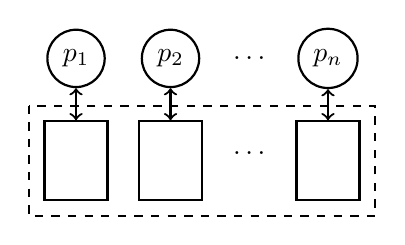
\begin{tikzpicture}
\node[circle, thick, draw] (v1) at (-0.2,0.8) {$p_1$};
\node[circle, thick, draw] (v3) at (1,0.8) {$p_2$};
\node (v7) at (2,0.8) {$\dots$};
\node at (2,-0.4) {$\dots$};
\node[circle, thick, draw] (v5) at (3,0.8) {$p_n$};

\node (v2) at (-0.2,-0.11) {};
\node (v4) at (1,-0.11) {};
\node (v6) at (3,-0.11) {};

\draw[thick] (-0.6,0) rectangle (0.2,-1);
\draw[thick]  (0.6,0) rectangle (1.4,-1);
\draw[thick]  (2.6,0) rectangle (3.4,-1);

\draw[<->, thick]  (v1) edge (v2);
\draw[<->, thick]  (v3) edge (v4);
\draw[<->, thick]  (v5) edge (v6);

\draw[thick, dashed]  (-0.8,0.2) rectangle (3.6,-1.2);
\end{tikzpicture}
		\label{fig:pgas}
	}
	$\hspace{36pt}$
	\subfloat[Hybrid PGAS+MPI] {
		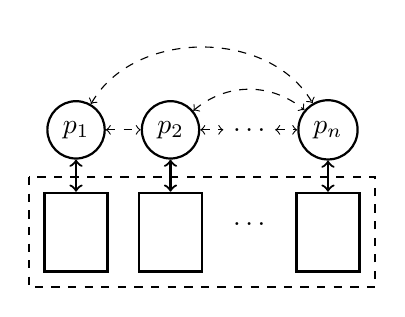
\begin{tikzpicture}
\node[circle, thick, draw] (v1) at (-0.2,0.8) {$p_1$};
\node[circle, thick, draw] (v3) at (1,0.8) {$p_2$};
\node (v7) at (2,0.8) {$\dots$};
\node at (2,-0.4) {$\dots$};
\node[circle, thick, draw] (v5) at (3,0.8) {$p_n$};

\node (v2) at (-0.2,-0.11) {};
\node (v4) at (1,-0.11) {};
\node (v6) at (3,-0.11) {};

\draw[thick] (-0.6,0) rectangle (0.2,-1);
\draw[thick]  (0.6,0) rectangle (1.4,-1);
\draw[thick]  (2.6,0) rectangle (3.4,-1);

\draw[<->, thick]  (v1) edge (v2);
\draw[<->, thick]  (v3) edge (v4);
\draw[<->, thick]  (v5) edge (v6);

\draw[thick, dashed]  (-0.8,0.2) rectangle (3.6,-1.2);

\draw[<->, dashed]  (v1) edge (v3);
\draw[<->, dashed]  (v3) edge (v7);
\draw[<->, dashed]  (v7) edge (v5);
\draw[<->, dashed]  (v3) edge [bend left=40 ] (v5) ;
\draw[<->, dashed]  (v1) edge [bend left=60 ] (v5);
\end{tikzpicture}
		\label{fig:pgas_hybrid}
	}
	\caption{Here $n$ processes $p_1, \dots, p_n$ are displayed in an \emph{PGAS} setting. Every process can access the entire combined memory, of which a small portion is local. The global address spaces are represented by dashed rectangles and the local address spaces by solid rectangles. }
	\label{fig:pgas_hybrid_pgas}
\end{figure}

\section{Partitioned Global Address Space}
The shared and distributed memory models can be combined into a \emph{distrbited shared memory} model. This is shown in Figure \ref{fig:pgas}. Every process has a local memory and all local memories are combined into a single global address space. This model is called \emph{Partitioned Global Address Space (PGAS)}, since the global address space is partitioned by the local memories of the participating processes. This makes PGAS a NUMA architecture.

PGAS combines most of the advantages of both the shared and distributed (SPMD) memory models. Data locality is exploited because every process knows its local memory. PGAS can be used both on a single computer and on a cluster of computers, because of its distributed structure. This simplifies programming systems to scale both parallel and distributed. 

\subsection{Asynchronous Partitioned Global Address Space}
A variant to PGAS is the \emph{Asynchronous Partitioned Global Address Space (APGAS)} model \cite{APGAS}. In APGAS the PGAS model is extended with tasks and task pools. Every node can asynchronously create and execute tasks both locally and remotely. Dynamic load-balancing is automatically applied over tasks. The PGAS model implicitly assumes all processes to run on similar hardware. APGAS has a richer execution framework due to its task-based structure and works well on non-uniform clusters.

\subsection{PGAS and MPI}
A \emph{Hybrid PGAS+MPI} parallel programming model can be used by combining PGAS with the distributed memory model. This is shown in Figure \ref{fig:pgas_hybrid}. In this model processes are able to perform message passing in addition to PGAS. The hybrid model can be used to implement software that does not entirely fit into the PGAS model. Also legacy code written for MPI can benefit from this model.

\subsection{PGAS and RDMA}
If PGAS is used in a distributed setting, it can be combined with RDMA. Every process creates an address space using virtual memory as an abstraction to the entire available memory. Local memory operations can simply be performed and remote operations are translated into one-sided RDMA operations. This makes the combination of RDMA and PGAS a high-performance parallel and distributed platform. 

\section{Parallel Programming Libraries}
This section introduces several parallel programming libraries that can be used in the research project.

\subsection{Message Passing Interface}
The \emph{Message Passing Interface (MPI)} is a popular interface for process communication written in C. With MPI processes can communicate by exchanging messages. MPI is used to create scalable parallel programs, as well as distributed programs.

MPI-3 supports one-sided communication and \emph{Remote Memory Access (RMA)} \cite{conf/sc/GerstenbergerBH13}, so MPI-3 is not longer limited to message passing alone. Many implementations of MPI-3 use RDMA when available to implement the one-sided operations and RMA. MPI also supports the shared memory model \cite{mpi-shared-mem-win}. 

\subsubsection{RMA and RDMA}
The difference between RMA and RDMA is that RDMA requires specialized hardware to directly access remote memory. Remote memory access can still be performed when RMDA-enabled hardware is not available by involving the OS kernel. MPI thus supports the use of remote memory calls without the need of specialized hardware by dropping the requirement of directly accessing remote memory. Many implementations of MPI however do use RDMA when the hardware enables it.

\subsubsection{MVAPICH2}
\emph{MVAPICH2} \cite{mvapich2} is an efficient implementation of MPI-3 for Infiniband hardware. It is efficient in the sense that hardware optimizations are used where possible. MVAPICH comes with a number of variants, one of which is \emph{MVAPICH2-X}, which supports PGAS and the hybrid PGAS/MPI model on Infiniband hardware. This implementation can be used with the PGAS models UPC and OpenSHMEM \cite{implementing_openshmem}. 

\subsubsection{PGAS and GPUs}
Another variant is \emph{MVAPICH2-GDR} \cite{Wang:2011:MOG:1997883.1997893}, which makes use of the GPUDirect RDMA technology \cite{gpudirect}. With MVAPICH2-GDR algorithms can be designed to operate on GPU clusters. It would be possible to design heterogeneous algorithms by combining MVAPICH2-X and MVAPICH2-GDR, but this is future work.

\subsection{PGAS Languages}
A number of PGAS languages exist, including Unified Parallel C (UPC), Co-array Fortran (CAF), Titanium, X10, Chapel, and OpenSHMEM. The languages UPC, CAS, and Titanium are extensions to C, Fortran, and Java, respectively. Since we are not planning to work with Fortran or Java, the languages CAS and Titanium are not discussed. 

\subsubsection{APGAS implementations}
Chapel and X10 are both implementations of the APGAS model \cite{Chamberlain:2007:PPC:1286120.1286123, Charles:2005:XOA:1103845.1094852}. Both are actual programming languages influenced by C++ and Java. These languages provide direct support for PGAS, task management and dynamic task load-balancing. A disadvantage is that the structure of both languages differs from C, so all existing BDD operations written in C have to be rewritten to X10 or Chapel if one of these languages is used. Also interoperability with LTSmin (or other existing tools) could be problematic, so these two languages are not discussed in this research project.

\subsubsection{OpenSHMEM}
OpenSHMEM (Open Shared Memory) is a specification for a standard API for parallel programming in PGAS \cite{openshmem}. Several implementations of OpenSHMEM exist, including an implementation for MVAPICH2-X. The performance of MVAPICH2-X in combination with OpenSHMEM is evaluated in \cite{openshmem_perf_evaluation} and compared to other OpenSHMEM libraries. The experiments were performed on the TACC Stampede cluster \cite{stampede_cluster}. The researchers concluded that this combination delivered best performance and scalability. Especially the atomic and collective operations performed significantly better due to the efficient use of Infiniband hardware. The atomic operations include \texttt{compare-and-swap} and \texttt{fetch-and-add} and the collective operations include \texttt{broadcast}, \texttt{reduce}, \texttt{collect}, and \texttt{barrier}. 

MVAPICH2-X can also be used in combination with UPC. Although this combination is not benchmarked in \cite{openshmem_perf_evaluation}, the benchmarks presented on the MVAPICH2 website show that UPC performs slightly better.

\section{Work Stealing}
Parallelization can be applied by dividing a big problem into smaller tasks so that multiple processes perform work simultaneously. The distribution of these tasks to processes is called \emph{load balancing}. In the ideal case, the work can be split perfectly into $n$ equal parts so that all $n$ processes receive an equal amount of work. In that case a speedup of $n$ can be achieved. However, this can not easily be done in practice, especially when the problem size is initially unknown. A number of different load balancing strategies exist that attempt to maximize speedup.

An efficient method to implement fine-grained task parallelism is \emph{work stealing}. In work stealing each process maintains a local task pool. Processes do not communicate with each other until they run out of tasks. In that case, the process attempts to steal work from other processes, then called \emph{victims}. The program terminates when all processes run out of tasks.

\subsection{Tasks}
A \emph{task} is a small part of a computation that only depends on its own intermediate \emph{subtasks} for its execution. When executing a task, it can create subtasks and later synchronize on those subtasks to complete the execution. Recursive algorithms can very easily be parallelized by using task-based parallelization, possibly in combination with a sort of cache to avoid redundant work. Since BDD operations are defined recursively, task-based parallelization can very well be applied to parallelize BDD operations, like shown in \cite{sylvan_multicore_bdd}.

Many task-based parallel frameworks like Cilk \cite{blumofe1996cilk}, Wool \cite{faxen2009wool}, and Lace \cite{lace} use the operations \texttt{spawn} and \texttt{sync} to spawn new tasks and synchronize on tasks, respectively. The \texttt{spawn} operation creates a new task and every task must be mached with a \texttt{sync} operation, like tasks are stored on a stack. The \texttt{sync} operation waits until the corresponding task completes and retrieves the results from that task. 

\begin{figure}
	\centering
	\begin{algorithm}[H]
		\SetStartEndCondition{ }{}{}%
		\SetKwProg{Fn}{int}{\string:}{}
		\SetKwFunction{fun}{fib}
		\SetKw{KwTo}{in}\SetKwFor{For}{for}{\string:}{}%
		\SetKwIF{If}{ElseIf}{Else}{if}{}{elif}{else}{}%
		\SetKwFor{While}{while}{:}{fintq}%
		\SetKw{test}{in}{}%
		\AlgoDontDisplayBlockMarkers\SetAlgoNoEnd\SetAlgoNoLine%

		\Fn{\fun{$n$}} {
			\textbf{if} $n < 2$ \textbf{return} $n$ \\
			\textbf{return} \texttt{fib}$(n-1)$ + \texttt{fib}$(n-2)$
		}
	\end{algorithm}

	\caption{The original recursive implementation of the Fibonacci function.}
	\label{fig:fib_seq}
\end{figure}

\begin{figure}
	\centering
	\begin{algorithm}[H]
		\SetStartEndCondition{ }{}{}%
		\SetKwProg{Fn}{int}{\string:}{}
		\SetKwFunction{fun}{par-fib}
		\SetKw{KwTo}{in}\SetKwFor{For}{for}{\string:}{}%
		\SetKwIF{If}{ElseIf}{Else}{if}{}{elif}{else}{}%
		\SetKwFor{While}{while}{:}{fintq}%
		\SetKw{test}{in}{}%
		\AlgoDontDisplayBlockMarkers\SetAlgoNoEnd\SetAlgoNoLine%

		\Fn{\fun{$n$}} {
			\textbf{if} $n < 2$ \textbf{return} $n$ \\
			\textbf{spawn}$(\texttt{par-fib}, \ n - 1)$ \\
			\textbf{spawn}$(\texttt{par-fib}, \ n - 2)$ \\
			$r \gets$ \textbf{sync} \\
			\textbf{return} $r \ + $ \textbf{sync}
		}
	\end{algorithm}

	\caption{The implementation of the Fibonacci function that uses fine-grained task-parallelism.}
	\label{fig:fib_par}
\end{figure}

Figure \ref{fig:fib_seq} shows the recursive implementation of the Fibonacci function. This implementation can easily be made parallel by performing the two recursive calls in parallel. Figure \ref{fig:fib_par} shows the same function, but now implemented with fine-grained task-parallelism. The two recursive calls now become subtasks and when both subtasks have completed (i.e. both \textbf{sync} operations yielded a result) the task itself completes. 

\begin{figure}
	\centering
	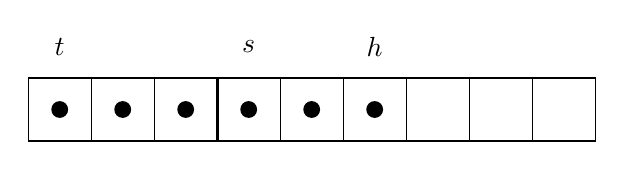
\begin{tikzpicture}[scale=0.8]
\draw[rectangle, draw]  (-1,0) rectangle (0,1);
\draw[rectangle, draw]  (0,0) rectangle (1,1);
\draw[rectangle, draw]  (1,0) rectangle (2,1) node (v1) {};
\draw[rectangle, draw]  (2,0) node (v2) {} rectangle (3,1);
\draw[rectangle, draw]  (3,0) rectangle (4,1);
\draw[rectangle, draw]  (4,0) rectangle (5,1);
\draw[rectangle, draw]  (5,0) rectangle (6,1);
\draw[rectangle, draw]  (6,0) rectangle (7,1);
\draw[rectangle, draw]  (7,0) rectangle (8,1);

\draw[rectangle, very thick, draw]  (2,-0) rectangle (2,1);

\node[circle, fill, draw, inner sep=2pt] at (-0.5,0.5) {};
\node[circle, fill, draw, inner sep=2pt] at (0.5,0.5) {};
\node[circle, fill, draw, inner sep=2pt] at (1.5,0.5) {};
\node[circle, fill, draw, inner sep=2pt] at (2.5,0.5) {};
\node[circle, fill, draw, inner sep=2pt] at (3.5,0.5) {};
\node[circle, fill, draw, inner sep=2pt] at (4.5,0.5) {};

\node at (-0.5,1.5) {$t$};
\node at (4.5,1.5) {$h$};
\node at (2.5,1.5) {$s$};

\end{tikzpicture}
	\caption{The split deque with a head $h$, a tail $t$, and a split point $s$. Here three items are added to the head of the queue and three items to the tail.}
	\label{fig:deque1}
\end{figure}

\begin{figure}
	\centering
	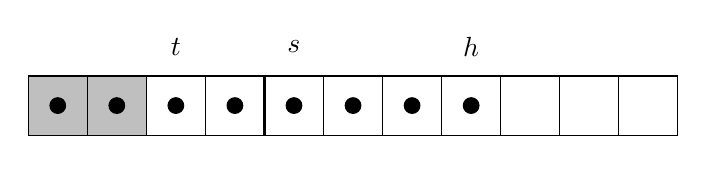
\begin{tikzpicture}[scale=0.75]
\draw[rectangle, color=black, fill=lightgray]  (-1,0) rectangle (0,1);
\draw[rectangle, color=black, fill=lightgray]  (0,0) rectangle (1,1);
\draw[rectangle, draw]  (1,0) rectangle (2,1) node (v1) {};
\draw[rectangle, draw]  (2,0) node (v2) {} rectangle (3,1);
\draw[rectangle, draw]  (3,0) rectangle (4,1);
\draw[rectangle, draw]  (4,0) rectangle (5,1);
\draw[rectangle, draw]  (5,0) rectangle (6,1);
\draw[rectangle, draw]  (6,0) rectangle (7,1);
\draw[rectangle, draw]  (7,0) rectangle (8,1);
\draw[rectangle, draw]  (8,0) rectangle (9,1);
\draw[rectangle, draw]  (9,0) rectangle (10,1);

\draw[rectangle, very thick, draw]  (3,-0) rectangle (3,1);

\node[circle, fill, draw, inner sep=2pt] at (-0.5,0.5) {};
\node[circle, fill, draw, inner sep=2pt] at (0.5,0.5) {};
\node[circle, fill, draw, inner sep=2pt] at (1.5,0.5) {};
\node[circle, fill, draw, inner sep=2pt] at (2.5,0.5) {};
\node[circle, fill, draw, inner sep=2pt] at (3.5,0.5) {};
\node[circle, fill, draw, inner sep=2pt] at (4.5,0.5) {};
\node[circle, fill, draw, inner sep=2pt] at (5.5,0.5) {};
\node[circle, fill, draw, inner sep=2pt] at (6.5,0.5) {};

\node at (1.5,1.5) {$t$};
\node at (6.5,1.5) {$h$};
\node at (3.5,1.5) {$s$};

\end{tikzpicture}
	\caption{The split deque in which every stolen element $x < t$ is made gray. Furthermore every element $x$ with $t < x < s$ belongs to the private part of the deque and every element $x \geq s$ belongs to the public part.}
	\label{fig:deque2}
\end{figure}

\subsection{Split Queues for Work Stealing}
The task pool can be implemented as a concurrent split deque \cite{lace}. A \emph{double ended queue (deque)} is similar to a queue, but has two ends, namely a head and a tail. Items can be \emph{pushed} and \emph{popped} from both ends of the deque. Unlike a normal queue, the deque does not require a LIFO or FIFO ordering. A \emph{split deque} is a deque that has a split point. Figure \ref{fig:deque1} shows an example of a split deque. The split point $s$ determines which part of the deque belongs to the head and which part to the tail. A head pointer $h$ and tail pointer $t$ determines the head and tail elements of the deque, respectively. A \emph{concurrent split deque} uses the \texttt{compare-and-swap} operation to enqueue and dequeue items from the split deque. 

The split deque can be splitted into a public and a private queue, where $s$ determines the border of the two queues. Every element $x < s$ belongs to the public queue and can be stolen by other processes. Every element $x \geq s$ belongs to the private queue and can only be accessed by the process owning the split deque. By stealing a task, the \emph{thief} pops an item from the public part of the \emph{victims} split deque and moves $t$ by using \texttt{compare-and-swap}. Thus every element $x < t$ is stolen. This is shown in Figure \ref{fig:deque2} where every element displayed in gray is stolen. 

The split point $s$ can be changed by the process owning the split deque. Changing $s$ can be done when the private part of the deque becomes empty or when it becomes very big. Thieves are not allowed to change $s$, since it would require an expensive memory fence. Instead, \cite{lace} suggests that a special flag \texttt{splitreq} is maintained by the process owning the split deque. The \texttt{splitreq} can be changed by thieves via \text{compare-and-swap} and the owner can check this flag before performing a \texttt{push} or \texttt{pop} operation. If the flag is set, the process moves $s$ so that the private part of the deque grows. Furthermore, the public part of the deque can also shrink by moving $s$ further into the public part. In that case, it could happen that $s < t$, which would mean that every element in the public part of the deque is already stolen. This can be avoided by using a \emph{memory fence} when shrinking the public queue.

A small improvement to work stealing is given in \cite{lace}, which suggests the use of an \texttt{allstolen} flag. This flag is set by the process owning the queue when it detects that all tasks in the public queue are stolen. Thieves can check this flag before attempting to steal a task, thus avoiding unnecessarily steal attempts. Also the owner can check this flag before shrinking the public queue in order to avoid unnecessarily shrinking.

\subsection{Victim Selection}
When a process needs to perform a \texttt{steal} operation, it needs to somehow find a victim. An obvious stategy is to select a victim randomly. Random victim selection appears to perform stable and has nice theoretical properties \cite{Blumofe:1998:PWS:277858.277939}. A disadvantage of random victim selection is that the size of task pools and the work distribution can fluctuate. This has a negative impact on scalability \cite{dinan2009scalable}. Furthermore a skew in the workload may lead to resources being wasted. 

Note that by stealing tasks, the thief performs work for the victim until the stolen task finishes. Now suppose that the victim steals back from the thief. Then the victim performs a part of the work that was stolen from him. This leads to a semi-random strategy called \emph{leapfrogging} \cite{Wagner:1993:LPT:173284.155354}, in which thieves are selected as victims in the process of victim selection. If there are no thieves, or when the thieves do not have any work in their public queue, a random victim is selected. This strategy ensures that the sizes of the task pools are more predictable. For example, Lace is making use of leapfrogging.

Varisteas et al. \cite{varisteas2014dvs} (published in 2014) introduces \emph{deterministic victim selection}, which removes all randomness. In this strategy each worker has a predefined partially ordered set of possible victims. Task distribution is done via a complex policy that achieves a uniform distribution. The researchers observed better scalability and an average performance improvement of $15\%$ compared to Wool.

\subsection{Implementation}
Simplified algorithms for the \texttt{spawn}, \texttt{sync}, and \texttt{steal} operations are given in \cite{lace}. This paper discusses a concurrent implementation of these operations as well as some improvements, but the simplified versions are enough to discuss the principles of work stealing.

\begin{figure}
	\centering
	\begin{algorithm}[H]
		\SetStartEndCondition{ }{}{}%
		\SetKwProg{Fn}{def}{\string:}{}
		\SetKwFunction{fun}{spawn}
		\SetKw{KwTo}{in}\SetKwFor{For}{for}{\string:}{}%
		\SetKwIF{If}{ElseIf}{Else}{if}{}{elif}{else}{}%
		\SetKwFor{While}{while}{:}{fintq}%
		\SetKw{test}{in}{}%
		\AlgoDontDisplayBlockMarkers\SetAlgoNoEnd\SetAlgoNoLine%

		\Fn{\fun{$t$}} {
			\textbf{self}.taskpool.\texttt{push}($t$)
		}
	\end{algorithm}

	\caption{A simple implementation of \texttt{spawn} that adds a task $t$ to a local task pool \cite{lace}.}
	\label{fig:workstealing_spawn}
\end{figure}

\begin{figure}
	\centering
	\begin{algorithm}[H]
		\SetStartEndCondition{ }{}{}%
		\SetKwProg{Fn}{def}{\string:}{}
		\SetKwFunction{fun}{sync}
		\SetKw{KwTo}{in}\SetKwFor{For}{for}{\string:}{}%
		\SetKwIF{If}{ElseIf}{Else}{if}{}{elif}{else}{}%
		\SetKwFor{While}{while}{:}{fintq}%
		\SetKw{test}{in}{}%
		\AlgoDontDisplayBlockMarkers\SetAlgoNoEnd\SetAlgoNoLine%

		\Fn{\fun{}} {
			$\langle s, t \rangle \gets$ \textbf{self}.taskpool.\texttt{pop}() \\
			\If{$s = $ \textbf{stolen}} {
				\While{$\neg t$.done} {
					\texttt{steal-work}($t.thief$)
				}
				$\langle s', t' \rangle \gets $ \textbf{self}.taskpool.\texttt{pop-stolen}() \\
				\Return{$t'$.result}
			}
			\textbf{return} $t.$\texttt{execute()}
		}
	\end{algorithm}

	\caption{A simple implementation of \texttt{sync} that uses leapfrogging \cite{lace}.}
	\label{fig:workstealing_sync}
\end{figure}

\begin{figure}
	\centering
	\begin{algorithm}[H]
		\SetStartEndCondition{ }{}{}%
		\SetKwProg{Fn}{def}{\string:}{}
		\SetKwFunction{fun}{steal-work}
		\SetKw{KwTo}{in}\SetKwFor{For}{for}{\string:}{}%
		\SetKwIF{If}{ElseIf}{Else}{if}{}{elif}{else}{}%
		\SetKwFor{While}{while}{:}{fintq}%
		\SetKw{test}{in}{}%
		\AlgoDontDisplayBlockMarkers\SetAlgoNoEnd\SetAlgoNoLine%

		\Fn{\fun{$v$}} {
			$t \gets v$.tasks.\texttt{steal()} \\
			\If{$\neg(t = \textbf{none})$} {
				$t$.thief = \textbf{self} \\
				$t$.result = $t$.\texttt{execute()} \\
				$t$.done = \textbf{true}
			}
		}
	\end{algorithm}

	\caption{A simple implementation of \texttt{steal-work} that attempts to steal from a victim $v$ \cite{lace}.}
	\label{fig:workstealing_steal}
\end{figure}

Figure \ref{fig:workstealing_spawn} shows a simple implementation of \texttt{spawn}. The \texttt{spawn} operation receives a task $t$ as a parameter and the operation adds it to the local taskpool of the executing process. 

Figure \ref{fig:workstealing_sync} shows an implementation of the \texttt{sync} operation. This operation simply pops a task $t$ with status $s$ from the task pool and executes it. If $t$ is a stolen task, the process continuously steals work from $t$s thief until $t$ completes, thus performing leapfrogging. 

Figure \ref{fig:workstealing_steal} shows the implementation of the \texttt{steal-work} operation. First the algorithm steals a task $t$ from a victim $v$. Stealing a task is performed by popping a task from the public (shared) part of $v$. If this succeeds, then $t$ is executed.

\subsection{Related Work}
Cilk and Wool \cite{blumofe1996cilk, faxen2009wool} are two task-based parallel frameworks. Cilk is a compiler-based framework, since it compiles programs written with Cilk to another form. Wool on the other hand is library-based. Cilk is relatively old (it appeared in 1996), and since the release of Cilk-5 \cite{frigo1998implementation} (appeared in 1998) work stealing can be performed with multiple threads. 

Lace \cite{lace} is a task-based parallel C library that uses non-blocking concurrent split deques. Lace also gives an implementation with private deques, because they solve some of the limitations of concurrent split deques. Experiments show that Lace is competitive with Wool and with the private deque algorithm. The paper also describes \emph{extended leapfrogging} that solves chaining problems that can arrise when using normal leapfrogging.

Palirria \cite{varisteas2014palirria} (published in 2014) is a work-stealing scheduling method for nested fork/join parallelism. Palirria comes with multiple implementations, including an implementation that uses the deterministic victim selection method and an implementation that has a resource estimation algorithm, which replaces the victim selection policy.